\documentclass[../main.tex]{subfiles}

\begin{document}

\subsection{Overview: High-level components and their interaction}
 TrackMe will be developed on a 3-tier architecture architecture \textit(Fig. 1), the rationale behind application servers separation is to mantain the Track4Help service
 aimed at companies, indipendent from AutomatedSOS and Track4Run functionalities, aimed at users. Application servers will interact with a database server.  Adding a layer of complexity with servers separation will  make 
 possible to handle failures and updates without the whole system going down.


  \begin{figure}[ht]
    \centering
         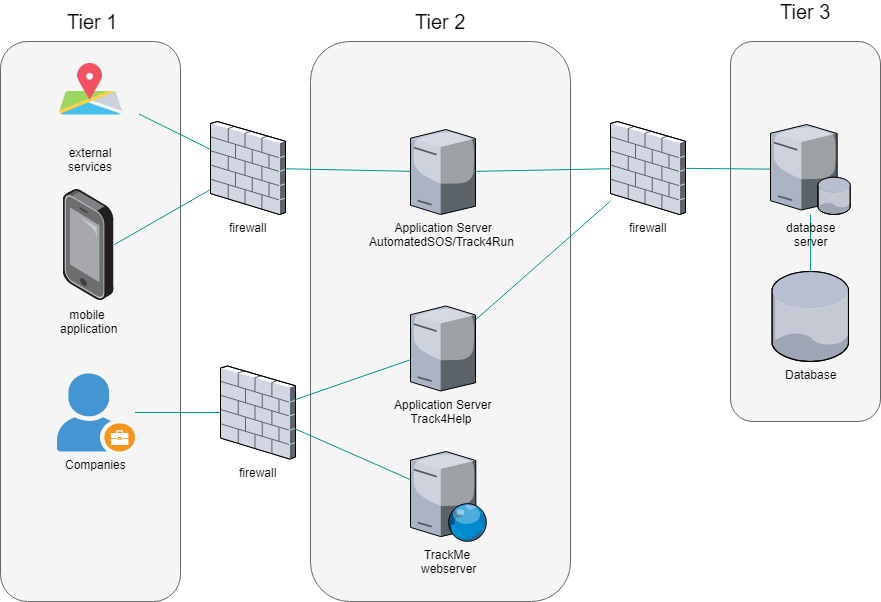
\includegraphics[width=1.0\textwidth]{trackme_architecture.png}
          \caption{TrackMe architecture}
           \label{fig:trackme_architecture}
    \end{figure}

    \begin{figure}[ht]
        \centering
             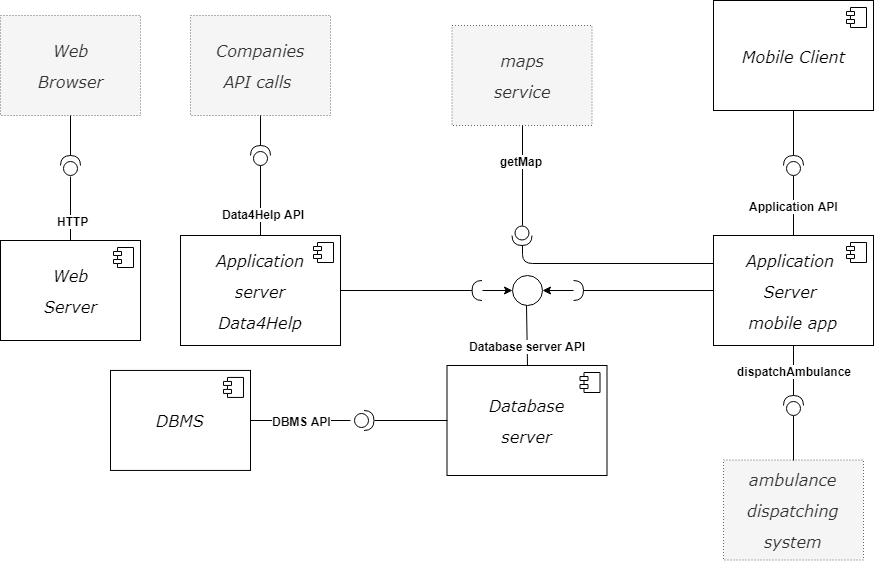
\includegraphics[width=1.0\textwidth]{high_level_component.png}
              \caption{High level components view}
               \label{fig:high_level_components}
        \end{figure}
 
\subsection{Component view}

\subsection{Deployment view}

\subsection{Runtime view}

\subsection{Component interfaces}

\subsection{Selected architectural styles and patterns}

\subsection{Other design decisions}

\end{document}
